\documentclass{beamer}
\usepackage{graphicx}
\usepackage{amsmath}
\usepackage{tikz}
\usepackage{setspace}
\usepackage{xcolor}
\usepackage{calc}
\usepackage{lmodern}
\usepackage[T1]{fontenc}
\usepackage{amsmath}


% \usepackage{tkz-graph} % Uncomment if needed
\DeclareMathOperator*{\argmax}{arg\,max}
% \usepackage{tkz-graph} % Uncomment if needed

% Theme
\usetheme{Madrid}
% Customizing colors
\definecolor{myred}{RGB}{180, 0, 0}
\definecolor{darkred}{RGB}{120, 0, 0}
\setbeamercolor{structure}{fg=myred}
\setbeamercolor{frametitle}{fg=white, bg=myred}
\setbeamercolor{title}{fg=white, bg=myred}
\setbeamercolor{block title}{fg=white, bg=gray!70!black}
\setbeamercolor{block body}{fg=black, bg=white}
\setbeamercolor{block title alerted}{fg=white, bg=darkred}
\setbeamercolor{block body alerted}{fg= black, bg=white}

% Remove borders from blocks
\setbeamertemplate{blocks}[default]
\setbeamercolor{block title}{fg=myred, bg=white}
\setbeamercolor{block body}{fg=black, bg=white}
\setbeamercolor{block title alerted}{fg=white, bg=darkred}
\setbeamercolor{block body alerted}{fg=black, bg=white}
\setbeamercolor{block title example}{fg=white, bg=myred}
\setbeamercolor{block body example}{fg=black, bg=white}

% No border lines around blocks
\setbeamertemplate{block alerted begin}{
    \par\vskip\medskipamount%
    \begin{beamercolorbox}[colsep*=.75ex,rounded=true,shadow=false]{block title alerted}%
        \usebeamerfont*{block title alerted}\insertblocktitle%
    \end{beamercolorbox}%
    {\parskip0pt\par}
    \begin{beamercolorbox}[colsep*=.75ex,rounded=true,shadow=false]{block body alerted}%
        \usebeamerfont{block body alerted}%
        \ignorespaces
} % ← This closes the \setbeamertemplate properly — no extra `}`

\setbeamertemplate{block alerted end}{
    \end{beamercolorbox}
    \vskip\smallskipamount
}


\setbeamertemplate{block example begin}{
    \par\vskip\medskipamount%
    \begin{beamercolorbox}[colsep*=.75ex,rounded=true,shadow=false]{block title example}%
        \usebeamerfont*{block title example}\insertblocktitle%
    \end{beamercolorbox}%
    {\parskip0pt\par}
    \begin{beamercolorbox}[colsep*=.75ex,rounded=true,shadow=false]{block body example}
        \usebeamerfont{block body example}
        \ignorespaces
}
\setbeamertemplate{block example end}{
    \end{beamercolorbox}
    \vskip\smallskipamount
}

\setbeamertemplate{block begin}{
    \par\vskip\medskipamount%
    \begin{beamercolorbox}[colsep*=.75ex,rounded=true,shadow=false]{block title}%
        \usebeamerfont*{block title}\insertblocktitle%
    \end{beamercolorbox}%
    {\parskip0pt\par}
    \begin{beamercolorbox}[colsep*=.75ex,rounded=true,shadow=false]{block body}
        \usebeamerfont{block body}
        \ignorespaces
}
\setbeamertemplate{block end}{
    \end{beamercolorbox}
    \vskip\smallskipamount
}


% Title Page
\title{Analysis of Algorithm}
\subtitle{Reductions Among Classic NP-Complete Problems: 3SAT, MIS, MVC, and 3-Colorability}
\author{Instructor: Dr. Mudassir Shabbir}
\institute{ITU}
\date{May 10, 2025}

\AtBeginDocument{
    \setbeamertemplate{logo}{%
        \hspace*{0.8\textwidth} % Adjust position
        
\includegraphics[width=1cm]{Itu.jpg} % Adjust size as needed
    }
}

\begin{document}
\begin{frame}
    \titlepage
    \vspace{1cm}
    \textbf{Scribe:}
 Abdul Basit  \\ \ \ \ \ \ \ \ \ \ \ \ Muhammad Okasha Khan
\end{frame}



\begin{frame}{\Large \textbf{What is Reduction?}}
    \begin{alertblock}{\textbf{Definition}}
        \textbf{Reduction} in algorithms is a technique where one problem is \textbf{translated into another problem} in such a way that a solution to the second problem can be used to solve the first one.
    \end{alertblock}

    \begin{alertblock}{\textbf{Reduction should be:}}
        \begin{itemize}
            \item Polynomial Time
            \item Translates yes instance to yes
            \item Translates no instance to no
            \item In $\rightarrow$ input of A, Out $\rightarrow$ input of B
        \end{itemize}
    \end{alertblock}
    \textbf{As we did 3-SAT $\leq_p$ MIS}
\end{frame}


\begin{frame}{Reduction Direction Matters}
    \textbf{Key Insight:} The difficulty of a reduction depends on its direction.
    
    \begin{itemize}
        \item Sorting $\leq_p$ 3SAT is easy.
        \item 3SAT $\leq_p$ Sorting would imply P = NP. (which is a big deal)
    \end{itemize}
    
    \begin{alertblock}{Computational Complexity Principle}
        If A $\leq_p$ B and B is in P, then A is in P. \\
        But if A is NP-complete and B is in P, then \textbf{P = NP}!
    \end{alertblock}
\end{frame}

\begin{frame}{Applications of Reduction}
    \begin{block}{\Large \textbf{Commonly Used In:}}
        \begin{itemize}
            \item {Algorithm Design}
            \item {Complexity Theory}
            \item {Problem Classification}
        \end{itemize}
    \end{block}
    \begin{block}{\large \textbf{Key Benefit}}
        Helps break complex problems into simpler or already-solved problems.
    \end{block}
\end{frame}

\begin{frame}{Reduction in Algorithm Design}
    \begin{exampleblock}{Example: Sorting $\rightarrow$ Selection}
        \begin{itemize}
            \item If you can repeatedly find the smallest element (selection)
            \item You can sort the entire list by:
            \begin{enumerate}
                \item Select minimum element
                \item Remove it from list
                \item Repeat until list is sorted
            \end{enumerate}
        \end{itemize}
    \end{exampleblock}
    
    \begin{alertblock}{Implementation}
        \texttt{SelectionSort} directly uses this reduction approach!
    \end{alertblock}
\end{frame}

\begin{frame}{Reduction in Complexity Theory}
    \textbf{\color{myred}{Proving Problem Hardness}}
        \[Used \ to \ compare \ difficulty \ of  \ problems, especially  \  for:\]
        \begin{itemize}
            \item NP-completeness proofs
            \item Undecidability proofs
        \end{itemize}
    
    \begin{exampleblock}{Standard Proof Technique}
        To show \textbf{Problem A} is hard:
        \begin{enumerate}
            \item Take a known hard problem (e.g., SAT)
            \item Reduce it to A in polynomial time
            \item Show solution to A solves SAT
            \item Conclude: A is at least as hard as SAT
        \end{enumerate}
    \end{exampleblock}

\end{frame}

\begin{frame}{Why Reduction Matters}
    \begin{columns}[T]
        \begin{column}{0.5\textwidth}
            \begin{block}{Practical Benefits}
                \begin{itemize}
                    \item \textbf{Algorithm Reuse}: Leverage existing solutions
                    \item \textbf{Optimal Design}: Build on proven strategies
                    \item \textbf{Code Efficiency}: Avoid reinventing the wheel
                \end{itemize}
            \end{block}
        \end{column}
        
        \begin{column}{0.5\textwidth}
            \begin{block}{Theoretical Importance}
                \begin{itemize}
                    \item \textbf{Hardness Proofs}: Classify problem difficulty
                    \textbf{Completeness}: Identify fundamental problems
                    \textbf{Computability}: Establish decidability limits
                \end{itemize}
            \end{block}
        \end{column}
    \end{columns}
\end{frame}

\begin{frame}{3-SAT Problem Definition}
    \begin{block}{What is 3-SAT?}
        A special case of the Boolean satisfiability problem (SAT), and one of the most famous \textbf{NP-complete} problems.
    \end{block}
    
    \begin{alertblock}{Key Characteristics}
        \begin{itemize}
            \item Boolean formula in \textbf{CNF} (Conjunctive Normal Form)
            \item Each clause has \textbf{exactly 3 literals}
            \item NP-complete (can verify solutions quickly, but no known efficient solution)
        \end{itemize}
        \textbf{\color{myred}{Decision Problem:}}
        "Is there a True/False assignment to variables that makes the entire formula evaluate to True?"
    \end{alertblock}
\end{frame}

\begin{frame}{Formal Definition of 3-SAT}
        \textbf{\color{myred}{Mathematical Representation}} \\
        \color{black}{Given a formula $\phi$ in 3-CNF form:}\\
         \centering $\phi = \bigwedge_{i=1}^m (l_{i1} \lor l_{i2} \lor l_{i3})$ \\
        \begin{flushleft} where:
            \begin{itemize}
                \item $m$ = number of clauses
                \item Each $l_{ij}$ is a \textbf{literal} (variable or its negation)
                \item $\land$ = AND (conjunction) $\lor$ = OR (disjunction)
            \end{itemize}

            \begin{alertblock}{Computational Challenge}
            The problem remains NP-complete even when:
                \begin{itemize}
                    \item No clause contains duplicate literals
                    \item Each variable appears in at most 3 clauses
                \end{itemize}
             \end{alertblock}
        \end{flushleft}
\end{frame}

\begin{frame}{3-SAT Example}
    \begin{exampleblock}{Sample 3-CNF Formula}
        \[
        (x_1 \lor \neg x_2 \lor x_3) \land (\neg x_1 \lor x_2 \lor x_4) \land (\neg x_3 \lor \neg x_4 \lor x_5)
        \]
    \end{exampleblock}
    
    \begin{columns}[T]
        \begin{column}{0.5\textwidth}
            \begin{block}{Components}
                \begin{itemize}
                    \item \textbf{Variables:} $x_1, x_2, x_3, x_4, x_5$
                    \item \textbf{Clauses:} 3
                    \item \textbf{Literals:} 9 (3 per clause)
                \end{itemize}
            \end{block}
        \end{column}
        
        \begin{column}{0.5\textwidth}
            \begin{alertblock}{Satisfying Assignment}
                One possible solution:
                \begin{itemize}
                    \item $x_1 =$ True
                    \item $x_2 =$ False
                    \item $x_3 =$ True
                    \item $x_4 =$ True
                    \item $x_5 =$ True
                \end{itemize}
            \end{alertblock}
        \end{column}
    \end{columns}
\end{frame}

\begin{frame}{Why 3-SAT Matters}
    \begin{block}{Theoretical Significance}
        \begin{itemize}
            \item \textbf{Canonical NP-complete problem}
            \item Used as starting point for thousands of NP-completeness proofs
            \item Fundamental in computational complexity theory
        \end{itemize}
    \end{block}
    
    \begin{alertblock}{Practical Applications}
        \begin{itemize}
            \item Circuit design verification
            \item AI planning problems
            \item Software verification
            \item Cryptography
        \end{itemize}
    \end{alertblock}
\end{frame}

\begin{frame}{3-SAT vs. General SAT}
    \begin{columns}[T]
        \begin{column}{0.5\textwidth}
            \begin{block}{3-SAT}
                \begin{itemize}
                    \item Every clause has \textbf{exactly 3 literals}
                    \item Still NP-complete
                    \item Often easier to reduce to
                    \item Standard benchmark problem
                \end{itemize}
            \end{block}
        \end{column}
        
        \begin{column}{0.5\textwidth}
            \begin{block}{General SAT}
                \begin{itemize}
                    \item Clauses can have \textbf{any number} of literals
                    \item First problem proven NP-complete (Cook-Levin)
                    \item More general but often reduced to 3-SAT
                \end{itemize}
            \end{block}
        \end{column}
    \end{columns}
    
    \begin{alertblock}{Key Theorem}
        Any NP problem can be \textbf{polynomially reduced} to 3-SAT while preserving satisfiability.
    \end{alertblock}
\end{frame}

\begin{frame}{3-SAT Example Walkthrough}
    \begin{exampleblock}{Given Formula}
        \[
        (x \lor y \lor z) \land (\neg x \lor \neg y) \land (x \lor \neg y \lor z)
        \]
        \textbf{Variables:} $x, y, z$ \\
        \textbf{Clauses:} 3 (corrected from original)
    \end{exampleblock}
    
    \textbf{\color{myred}{Verification Process:}} \\
        \textbf{Try assignment:} $x=\text{True}, y=\text{False}, z=\text{True}$
        
        \begin{enumerate}
            \item $(T \lor F \lor T) \equiv T$
            \item $(\neg T \lor \neg F) \equiv (F \lor T) \equiv T$
            \item $(T \lor \neg F \lor T) \equiv (T \lor T \lor T) \equiv T$
        \end{enumerate}
        
        \textbf{Result:} All clauses satisfied → Formula is satisfiable
    
    \textbf{\color{myred}{Note on Original Example:}} \\
        The original formula contained a 4-literal clause $(y \lor x \lor y \lor z)$ which violates 3-SAT rules. This has been corrected.
\end{frame}

\begin{frame}{Vertex Cover Problem}
    \begin{block}{Definition}
        A \textbf{vertex cover} of a graph $G=(V,E)$ is a subset $C \subseteq V$ such that:
        \[
        \forall (u,v) \in E,\; u \in C \;\lor\; v \in C
        \]
    \end{block}
    
    \begin{columns}[T]
        \begin{column}{0.5\textwidth}
            \begin{alertblock}{Decision Problem}
                \textbf{Input:} Graph $G$ and integer $k$ \\
                \textbf{Question:} Does $G$ have a vertex cover of size $\leq k$?
            \end{alertblock}
            
            \end{column}
        
        \begin{column}{0.5\textwidth}
            \begin{center}
                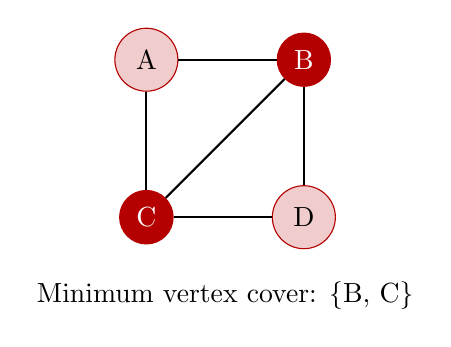
\begin{tikzpicture}[
                    node/.style={circle, draw=myred, fill=myred!20, minimum size=8mm},
                    selected/.style={circle, draw=myred, fill=myred, text=white},
                    edge/.style={draw, thick}
                ]
                    \node[node] (a) at (0,2) {A};
                    \node[selected] (b) at (2,2) {B};
                    \node[selected] (c) at (0,0) {C};
                    \node[node] (d) at (2,0) {D};
                    
                    \draw[edge] (a) -- (b);
                    \draw[edge] (a) -- (c);
                    \draw[edge] (b) -- (c);
                    \draw[edge] (b) -- (d);
                    \draw[edge] (c) -- (d);
                    
                    \node at (1,-1) {Minimum vertex cover: \{B, C\}};
                \end{tikzpicture}
            \end{center}
        \end{column}
    \end{columns}
\end{frame}

\begin{frame}{Vertex Cover Properties}
    \begin{exampleblock}{Simple Algorithm}
        \begin{enumerate}
            \item While edges remain:
            \begin{itemize}
                \item Pick any edge $(u,v)$
                \item Add both $u$ and $v$ to cover
                \item Remove all edges incident to $u$ or $v$
            \end{itemize}
            \item Output the selected vertices
        \end{enumerate}
    \end{exampleblock}
    
    \begin{alertblock}{Note}
        This greedy algorithm doesn't give minimal cover but guarantees $|C| \leq 2 \times$ optimal
    \end{alertblock}
\end{frame}

\begin{frame}{Vertex Cover Example}
            \begin{block}{Graph Instance}
            \centering
                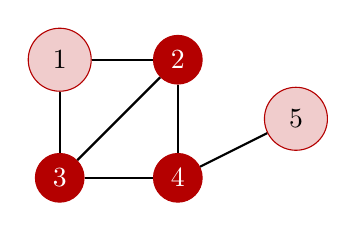
\begin{tikzpicture}[
                    node/.style={circle, draw=myred, fill=myred!20, minimum size=8mm},
                    selected/.style={circle, draw=myred, fill=myred, text=white},
                    edge/.style={draw, thick}
                ]
                    \node[node] (1) at (0,1.5) {1};
                    \node[selected] (2) at (1.5,1.5) {2};
                    \node[selected] (3) at (0,0) {3};
                    \node[selected] (4) at (1.5,0) {4};
                    \node[node] (5) at (3,0.75) {5};
                    
                    \draw[edge] (1) -- (2);
                    \draw[edge] (1) -- (3);
                    \draw[edge] (2) -- (3);
                    \draw[edge] (2) -- (4);
                    \draw[edge] (3) -- (4);
                    \draw[edge] (4) -- (5);
                \end{tikzpicture}
                \begin{itemize}
                    \item \textcolor{myred}{\{2,3,4\}} (size 3)
                    \item \{1,3,4\} (size 3)
                    \item \{2,3,5\} (size 3)
                \end{itemize}
            \end{block}
            
\end{frame}

\begin{frame}{Types of Vertex Cover Problems}
    \begin{columns}[T]
        \begin{column}{0.7\textwidth}
            \begin{block}{Decision Problem}
                \textbf{Input:} 
                \begin{itemize}
                    \item Graph $G=(V,E)$
                    \item Integer $k$
                \end{itemize}
                \textbf{Question:} \\
                Does $G$ have a vertex cover of size $\leq k$?
                
                \begin{center}
                    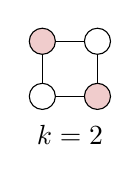
\begin{tikzpicture}[scale=0.7]
                        \node[draw,circle,fill=myred!20] (a) at (0,1) {};
                        \node[draw,circle] (b) at (1,1) {};
                        \node[draw,circle] (c) at (0,0) {};
                        \node[draw,circle ,fill=myred!20] (d) at (1,0) {};
                        \draw (a) -- (b) -- (d) -- (c) -- (a);
                        \node at (0.5,-0.7) {$k=2$};
                    \end{tikzpicture}
                \end{center}
            \end{block}
        \end{column}
        
        \begin{column}{0.3\textwidth}
            \begin{block}{Optimization Problem}
                \textbf{Input:} Graph $G=(V,E)$ \\
                \textbf{Goal:} Find the \textcolor{myred}{minimum} vertex cover $C^*$
                
                \begin{center}
                    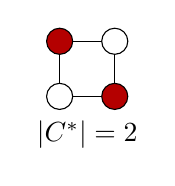
\begin{tikzpicture}[scale=0.7]
                        \node[draw,circle,fill=myred] (a) at (0,1) {};
                        \node[draw,circle] (b) at (1,1) {};
                        \node[draw,circle] (c) at (0,0) {};
                        \node[draw,circle,fill=myred] (d) at (1,0) {};
                        \draw (a) -- (b) -- (d) -- (c) -- (a);
                        \node at (0.5,-0.7) {$|C^*|=2$};
                    \end{tikzpicture}
                \end{center}
            \end{block}
        \end{column}
    \end{columns}
    \textbf{Equivalence:}
        The decision version is NP-complete $\iff$ The optimization version is NP-hard
\end{frame}

\begin{frame}{Maximum Independent Set (MIS)}
    \begin{block}{Definition}
        Given an undirected graph $G=(V,E)$, an \textbf{independent set} is a subset $S \subseteq V$ where:
        \[
        \forall u,v \in S,\; (u,v) \notin E
        \]
        The \textcolor{myred}{Maximum} Independent Set is the largest such $S$.
    \end{block}
    
    \begin{columns}[T]
        \begin{column}{0.5\textwidth}
            \begin{alertblock}{Decision Problem}
                \textbf{Input:} Graph $G$, integer $k$ \\
                \textbf{Question:} Does $G$ have an independent set of size $\geq k$?
            \end{alertblock}
        \end{column}
        \begin{column}{0.5\textwidth}
            \begin{exampleblock}{Optimization Problem}
                Find the independent set with maximum cardinality:
                \centering $S^* = \argmax_{S \subseteq V} |S|$
            \end{exampleblock}
        \end{column}
    \end{columns}
\end{frame}

\begin{frame}{Maximum Independant Set}
    \begin{center}
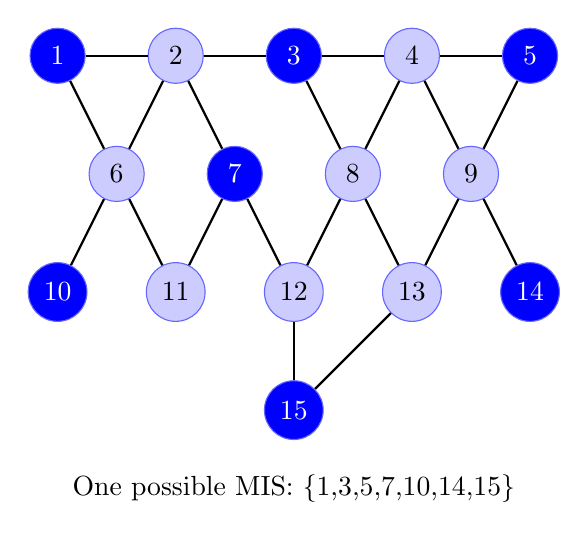
\begin{tikzpicture}[
    node/.style={circle, draw=blue!60, fill=blue!20, minimum size=7mm},
    selected/.style={circle, draw=blue!60, fill=blue, text=white, minimum size=7mm},
    edge/.style={draw, thick}
]

% Row 1
\node[selected] (1) at (0,0) {1};
\node[node] (2) at (1.5,0) {2};
\node[selected] (3) at (3,0) {3};
\node[node] (4) at (4.5,0) {4};
\node[selected] (5) at (6,0) {5};

% Row 2
\node[node] (6) at (0.75,-1.5) {6};
\node[selected] (7) at (2.25,-1.5) {7};
\node[node] (8) at (3.75,-1.5) {8};
\node[node] (9) at (5.25,-1.5) {9};

% Row 3
\node[selected] (10) at (0,-3) {10};
\node[node] (11) at (1.5,-3) {11};
\node[node] (12) at (3,-3) {12};
\node[node] (13) at (4.5,-3) {13};
\node[selected] (14) at (6,-3) {14};

% Row 4
\node[selected] (15) at (3,-4.5) {15};

% Edges
\foreach \i/\j in {1/2, 2/3, 3/4, 4/5, 1/6, 2/6, 2/7, 3/8, 4/8, 4/9, 5/9,
                   6/10, 6/11, 7/11, 7/12, 8/12, 8/13, 9/13, 9/14,
                   12/15, 13/15}
    \draw[edge] (\i) -- (\j);

% MIS label
\node at (3,-5.5) {One possible MIS: \{1,3,5,7,10,14,15\}};

\end{tikzpicture}

    \end{center}
\end{frame}

\begin{frame}{Reduction: MIS $\leq_p$ MVC}
    \color{myred}{Objective} \\
        \color{black}{Transform any MIS instance into an MVC instance such that:}
        \[
        S \text{ is MIS of } G \iff V\setminus S \text{ is MVC of } G
        \]
    
    \begin{columns}[T]
        \begin{column}{0.5\textwidth}
            \begin{alertblock}{Reduction Steps}
                \begin{enumerate}
                    \item Start with graph $G=(V,E)$ for MIS
                    \item Use \textbf{same graph} for MVC
                    \item Let $k = |V| - t$ (where $t$ is target MIS size)
                    \item Solve MVC$(G, k)$
                    \item Return $V \setminus C$ as MIS
                \end{enumerate}
            \end{alertblock}
        \end{column}
        
        \begin{column}{0.5\textwidth}
            \begin{center}
                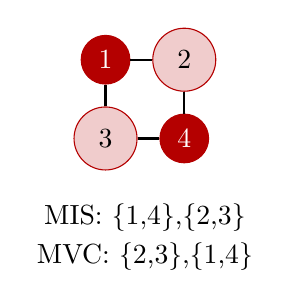
\begin{tikzpicture}[
                    node/.style={circle, draw=myred, fill=myred!20, minimum size=8mm},
                    selected/.style={circle, draw=myred, fill=myred, text=white},
                    edge/.style={draw, thick}
                ]
                    \node[selected] (1) at (0,1) {1};
                    \node[node] (2) at (1,1) {2};
                    \node[node] (3) at (0,0) {3};
                    \node[selected] (4) at (1,0) {4};
                    
                    \draw[edge] (1) -- (2) -- (4) -- (3) -- (1);
                    
                    \node at (0.5,-1) {MIS: \{1,4\},\{2,3\}};
                    \node at (0.5,-1.5) {MVC: \{2,3\},\{1,4\}};
                \end{tikzpicture}
            \end{center}
        \end{column}
    \end{columns}
\end{frame}

\begin{frame}{Proof of Correctness}
    \color{red}{Key Lemma:} \\
        \color{black}{For any graph $G=(V,E)$ and subset $S \subseteq V$:}
        \[
        S \text{ is independent set} \iff V\setminus S \text{ is vertex cover}
        \]
        An independent set is a set of vertices with no two adjacent. \\
A vertex cover is a set of vertices that touches every edge (i.e. every edge has at least one endpoint in the set).

    \color{red}{Proof:}
        \begin{itemize}
            \item ($\Rightarrow$) If $S$ is independent, every edge has $\geq 1$ endpoint in $V\setminus S$ (else $S$ wouldn't be independent)
            \item ($\Leftarrow$) If $V\setminus S$ is vertex cover, no edge connects two vertices in $S$ (else $V\setminus S$ wouldn't cover it)
        \end{itemize}
    
    \color{red}{Implications:}
        \begin{itemize}
            \item Size relationship: $|S| = |V| - |C|$
            \item $S$ is maximum independent set $\iff$ $C$ is minimum vertex cover
            \item Reduction preserves optimality
        \end{itemize}
\end{frame}

\begin{frame}{Example Reduction}
    \begin{columns}[T]
        \begin{column}{0.5\textwidth}
            \textbf{\color{myred}{Original Graph $G$}} \\[1ex]
            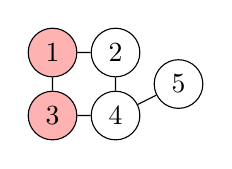
\begin{tikzpicture}[scale=0.8, every node/.style={circle, draw, minimum size=6mm}]
                \node[fill=red!30] (1) at (0,1) {1};
                \node (2) at (1,1) {2};
                \node[fill=red!30] (3) at (0,0) {3};
                \node (4) at (1,0) {4};
                \node (5) at (2,0.5) {5};
                
                \draw (1) -- (2) -- (4) -- (3) -- (1);
                \draw (4) -- (5);
            \end{tikzpicture} \\[1ex]

            \textbf{MIS Instance:}
            \begin{itemize}
                \item $V = \{1,2,3,4,5\}$
                \item Target size $t = 2$
            \end{itemize}
        \end{column}
        
        \begin{column}{0.5\textwidth}
            \textbf{\color{myred}{Reduced MVC Instance}} \\[1ex]
            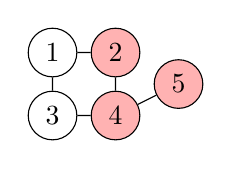
\begin{tikzpicture}[scale=0.8, every node/.style={circle, draw, minimum size=6mm}]
                \node (1) at (0,1) {1};
                \node[fill=red!30] (2) at (1,1) {2};
                \node (3) at (0,0) {3};
                \node[fill=red!30] (4) at (1,0) {4};
                \node[fill=red!30] (5) at (2,0.5) {5};
                
                \draw (1) -- (2) -- (4) -- (3) -- (1);
                \draw (4) -- (5);
            \end{tikzpicture} \\[1ex]

            \textbf{Parameters:}
            \begin{itemize}
                \item Same graph $G$
                \item $k = |V| - t = 3$
            \end{itemize}
        \end{column}
    \end{columns}
    
    \begin{exampleblock}{Solution Mapping}
        \begin{itemize}
            \item MVC solution: $\{2,4,5\}$ (size 3)
            \item MIS solution: $V \setminus \{2,4,5\} = \{1,3\}$
            \item Verification: $\{1,3\}$ is indeed an independent set
        \end{itemize}
    \end{exampleblock}
\end{frame}


\begin{frame}{Complexity Implications}
    \begin{block}{Reduction Properties}
        \begin{itemize}
            \item \textbf{Time:} $O(1)$ (graph remains unchanged)
            \item \textbf{Space:} No additional memory needed
            \item \textbf{Approximation:} Preserves approximation ratios
        \end{itemize}
    \end{block}
    
    \begin{alertblock}{Theoretical Consequences}
        \begin{itemize}
            \item Since MIS is NP-hard, MVC must also be NP-hard
            \item MVC inherits inapproximability results from MIS
            \item Any algorithm for MVC can solve MIS via this reduction
        \end{itemize}
    \end{alertblock}
    
    
\end{frame}

\begin{frame}{Graph Colorability Problem}
    \textbf{\color{myred}{Definition}}
        A graph $G=(V,E)$ is \textbf{$k$-colorable} if there exists a function:
        \[
        c : V \rightarrow \{1,2,\dots,k\}
        \]
        such that:
        \[
        \forall (u,v) \in E,\; c(u) \neq c(v)
        \]
    
    \begin{columns}[T]
        \begin{column}{0.5\textwidth}
            \begin{alertblock}{Decision Problem}
                \textbf{Input:} Graph $G$, integer $k$ \\
                \textbf{Question:} Is $G$ $k$-colorable?
            \end{alertblock}
            
            \textbf{\color{myred}{Optimization Version}}
                Find the \textcolor{myred}{chromatic number} $\chi(G)$: \\
                The smallest $k$ for which $G$ is $k$-colorable
        \end{column}
        
        \begin{column}{0.5\textwidth}
            \begin{center}
                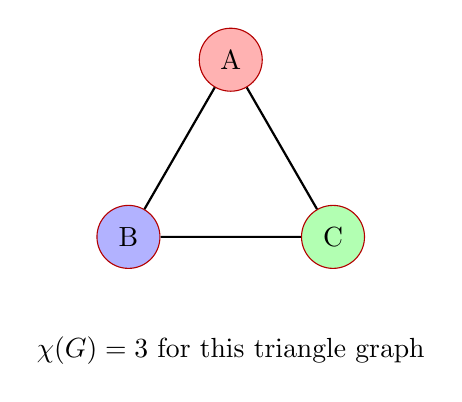
\begin{tikzpicture}[
                    node/.style={circle, draw=myred, fill=myred!20, minimum size=8mm},
                    edge/.style={draw, thick}
                ]
                    \node[node, fill=red!30] (A) at (90:1.5) {A};
                    \node[node, fill=blue!30] (B) at (210:1.5) {B};
                    \node[node, fill=green!30] (C) at (330:1.5) {C};
                    
                    \draw[edge] (A) -- (B) -- (C) -- (A);
                    
                    \node at (0,-2.2) {$\chi(G)=3$ for this triangle graph};
                \end{tikzpicture}
            \end{center}
        \end{column}
    \end{columns}
\end{frame}

\begin{frame}{Colorability Examples}
    \begin{columns}[T]
        \begin{column}{0.5\textwidth}
            \textbf{\color{myred}{2-Colorable Graphs}}
                \begin{itemize}
                    \item Bipartite graphs
                    \item Trees
                    \item Even-length cycles
                \end{itemize}
                
                \begin{center}
                    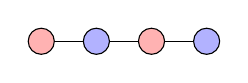
\begin{tikzpicture}[scale=0.7]
                        \node[circle, draw, fill=red!30] (1) at (0,0) {};
                        \node[circle, draw, fill=blue!30] (2) at (1,0) {};
                        \node[circle, draw, fill=red!30] (3) at (2,0) {};
                        \node[circle, draw, fill=blue!30] (4) at (3,0) {};
                        \draw (1) -- (2) -- (3) -- (4);
                    \end{tikzpicture}
                \end{center}
        \end{column}
        
        \begin{column}{0.5\textwidth}
            \textbf{\color{myred}{Non-2-Colorable}}
                \begin{itemize}
                    \item Odd-length cycles
                    \item Complete graphs ($K_n$ needs $n$ colors)
                \end{itemize}
                
                \begin{center}
                    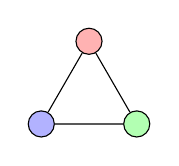
\begin{tikzpicture}[scale=0.7]
                        \node[circle, draw, fill=red!30] (1) at (90:1) {};
                        \node[circle, draw, fill=blue!30] (2) at (210:1) {};
                        \node[circle, draw, fill=green!30] (3) at (330:1) {};
                        \draw (1) -- (2) -- (3) -- (1);
                    \end{tikzpicture}
                \end{center}
        \end{column}
    \end{columns}
    
    \begin{alertblock}{Testing 2-Colorability}
        Equivalent to checking if the graph is \textbf{bipartite} - solvable in $O(|V|+|E|)$ time using BFS/DFS
    \end{alertblock}
\end{frame}

\begin{frame}{Graph Coloring Complexity}
    \textbf{\color{myred}{Theoretical Status}}
        \begin{itemize}
            \item \textbf{2-Coloring}: Polynomial time (bipartite check)
            \item \textbf{3-Coloring}: NP-complete (reducible from 3-SAT)
            \item \textbf{$k$-Coloring ($k \geq 3$)}: NP-complete
            \item \textbf{Approximation}: No constant factor approximation unless P=NP
        \end{itemize}
    
    \begin{columns}[T]
        \begin{column}{0.6\textwidth}
            \begin{exampleblock}{Greedy Coloring Algorithm}
                \begin{enumerate}
                    \item Order vertices arbitrarily
                    \item For each vertex:
                    \begin{itemize}
                        \item Assign smallest available color not used by neighbors
                    \end{itemize}
                    \item Uses $\leq \Delta+1$ colors ($\Delta$ = maximum degree)
                \end{enumerate}
            \end{exampleblock}
        \end{column}
        
        \begin{column}{0.4\textwidth}
            \begin{center}
                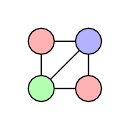
\begin{tikzpicture}[scale=0.6]
                    \node[circle, draw, fill=red!30] (1) at (0,1) {};
                    \node[circle, draw, fill=blue!30] (2) at (1,1) {};
                    \node[circle, draw, fill=green!30] (3) at (0,0) {};
                    \node[circle, draw, fill=red!30] (4) at (1,0) {};
                    \draw (1) -- (2) -- (4) -- (3) -- (1);
                    \draw (2) -- (3);
                \end{tikzpicture}
            \end{center}
        {\singlespacing}
        \textbf{\color{myred}{Brooks' Theorem:}} \\
        \color{black}{Any connected graph is $\Delta$-colorable, except complete graphs and odd cycles}
        \end{column}
    \end{columns}
\end{frame}

\begin{frame}{Special Cases and Variants}
    \begin{columns}[T]
        \begin{column}{0.5\textwidth}
            \textbf{\color{myred}{Edge Coloring}}
                \begin{itemize}
                    \item Color edges instead of vertices
                    \item No adjacent edges share color
                    \item Vizing's Theorem: $\Delta \leq \chi'(G) \leq \Delta+1$
                \end{itemize}
                
            \textbf{\color{myred}{List Coloring}}
                \begin{itemize}
                    \item Each vertex has its own set of allowed colors
                    \item More general than classic coloring
                \end{itemize}
        \end{column}
        
        \begin{column}{0.5\textwidth}
            \begin{alertblock}{Perfect Graphs}
                \begin{itemize}
                    \item $\chi(G) = \omega(G)$ (clique number)
                    \item Includes:
                    \begin{itemize}
                        \item Bipartite graphs
                        \item interval graphs
                        \item Chordal graphs
                    \end{itemize}
                \end{itemize}
            \end{alertblock}
            
            \begin{center}
                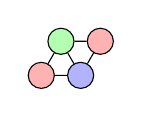
\begin{tikzpicture}[scale=0.5]
                    \node[circle, draw, fill=red!30] (1) at (0,0) {};
                    \node[circle, draw, fill=blue!30] (2) at (1,0) {};
                    \node[circle, draw, fill=green!30] (3) at (0.5,0.866) {};
                    \draw (1) -- (2) -- (3) -- (1);
                    \node[circle, draw, fill=red!30] (4) at (1.5,0.866) {};
                    \draw (2) -- (4) -- (3);
                \end{tikzpicture}
            \end{center}
        \end{column}
    \end{columns}
    
    \textbf{\color{myred}{Four Color Theorem:}} \\
        Every planar graph is 4-colorable (famous mathematical result proved in 1976)

\end{frame}

\begin{frame}{3-SAT $\leq_p$ 3-Coloring Reduction}
    \textbf{\color{myred}{Objective}} \\
        Given a 3-CNF formula $\Phi$, construct graph $G_\Phi$ such that:
        \[
        \Phi \text{ is satisfiable} \iff G_\Phi \text{ is 3-colorable}
        \]

    \begin{columns}[T]
        \begin{column}{0.5\textwidth}
            \textbf{\color{myred}{Color Semantics:}}
                \begin{itemize}
                    \item \textcolor{green}{T} (True)
                    \item \textcolor{red}{F} (False)
                    \item \textcolor{blue}{N} (Base)
                \end{itemize}

            \textbf{\color{myred}{Key Components:}}
                \begin{itemize}
                    \item Variable gadgets
                    \item Clause gadgets
                    \item Coloring constraints
                \end{itemize}
        \end{column}

        \begin{column}{0.5\textwidth}
            \begin{center}
                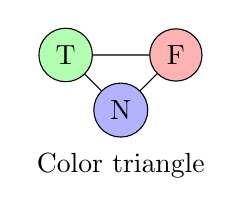
\begin{tikzpicture}[scale=0.7]
                    \node[draw,circle,fill=blue!30] (N) at (0,0) {N};
                    \node[draw,circle,fill=green!30] (T) at (-1,1) {T};
                    \node[draw,circle,fill=red!30] (F) at (1,1) {F};
                    \draw (N) -- (T) -- (F) -- (N);
                    \node at (0,-1) {Color triangle};
                \end{tikzpicture}
            \end{center}
        \end{column}
    \end{columns}
\end{frame}

\begin{frame}{Variable Gadget Construction}
    \begin{columns}[T]
        \begin{column}{0.6\textwidth}
            \textbf{\color{myred}{For each variable $x_i$}}
                \begin{itemize}
                    \item Create triangle: $x_i$, $\neg x_i$, and common vertex $N$
                    \item Forces $x_i$ and $\neg x_i$ to be T/F (opposite colors)
                    \item Base vertex enforces constraints
                \end{itemize}

            \textbf{\color{myred}{Coloring Implications}}
                \begin{itemize}
                    \item If $x_i$ = \textcolor{green}{T}, then $\neg x_i$ = \textcolor{red}{F}
                    \item If $x_i$ = \textcolor{red}{F}, then $\neg x_i$ = \textcolor{green}{T}
                \end{itemize}
            {\doublespacing}
            \textbf{\color{myred}{Example Assignment}}
        \end{column}

        \begin{column}{0.4\textwidth}
            \begin{center}
                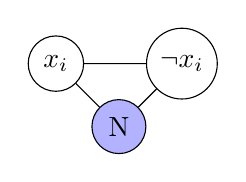
\begin{tikzpicture}[scale=0.8]
                    \node[draw,circle,fill=blue!30] (N) at (1,0) {N};
                    \node[draw,circle] (x) at (0,1) {$x_i$};
                    \node[draw,circle] (nx) at (2,1) {$\neg x_i$};
                    \draw (N) -- (x) -- (nx) -- (N);
                \end{tikzpicture}
            \end{center}
            
        \end{column}
    \end{columns}
        \begin{center}
            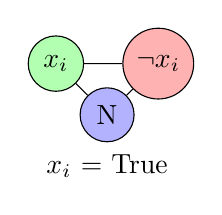
\begin{tikzpicture}[scale=0.65]
                \node[draw,circle,fill=blue!30] (N) at (1,0) {N};
                \node[draw,circle,fill=green!30] (x) at (0,1) {$x_i$};
                \node[draw,circle,fill=red!30] (nx) at (2,1) {$\neg x_i$};
                \draw (N) -- (x) -- (nx) -- (N);
                \node at (1,-1) {$x_i$ = True};
            \end{tikzpicture}
        \end{center}
\end{frame}

\begin{frame}{Clause Gadget Construction}
    \begin{columns}[T]
        \begin{column}{0.6\textwidth}
            \textbf{\color{myred}{For each clause $(l_1 \lor l_2 \lor l_3)$}}
                \begin{itemize}
                    \item Create triangle connecting literals to new vertex $C$
                    \item Add edge to base vertex $B$
                    \item Ensures at least one literal is \textcolor{green}{T}
                \end{itemize}
            
        \end{column}

        \begin{column}{0.4\textwidth}
            \begin{center}
                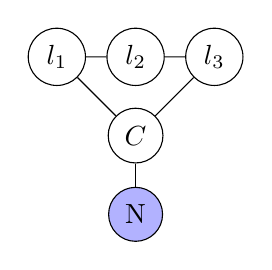
\begin{tikzpicture}[scale=1.0]
                    \node[draw,circle,fill=blue!30] (N) at (1,-1) {N};
                    \node[draw,circle] (l1) at (0,1) {$l_1$};
                    \node[draw,circle] (l2) at (1,1) {$l_2$};
                    \node[draw,circle] (l3) at (2,1) {$l_3$};
                    \node[draw,circle] (C) at (1,0) {$C$};
                    \draw (N) -- (C);
                    \draw (C) -- (l1) -- (l2) -- (l3) -- (C);
                \end{tikzpicture}
            \end{center}
        \end{column}
    \end{columns}
    \textbf{\color{myred}{Satisfaction Condition}}
                A clause gadget is properly colored iff at least one literal vertex is \textcolor{green}{T}
            
    \textbf{\color{myred}{Valid Coloring: }} \color{black}{Clause satisfied by $l_2$}
            \begin{center}
                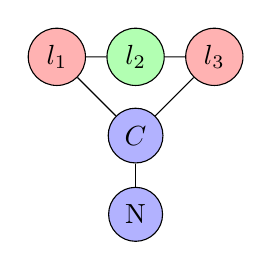
\begin{tikzpicture}[scale=1.0]
                    \node[draw,circle,fill=blue!30] (N) at (1,-1) {N};
                    \node[draw,circle,fill=red!30] (l1) at (0,1) {$l_1$};
                    \node[draw,circle,fill=green!30] (l2) at (1,1) {$l_2$};
                    \node[draw,circle,fill=red!30] (l3) at (2,1) {$l_3$};
                    \node[draw,circle,fill=blue!30] (C) at (1,0) {$C$};
                    \draw (N) -- (C);
                    \draw (C) -- (l1) -- (l2) -- (l3) -- (C);
                \end{tikzpicture}
            \end{center}
\end{frame}

\begin{frame}{Full Construction Example}
    \begin{block}{For formula $(x_1 \lor \neg x_2 \lor x_3) \land (\neg x_1 \lor x_2 \lor x_4)$}
    \begin{enumerate}
        \item Build variable gadgets for $x_1$ to $x_4$
        \item Connect literals to clause gadgets
        \item Add base vertex connections
    \end{enumerate}
\end{block}

\begin{center}
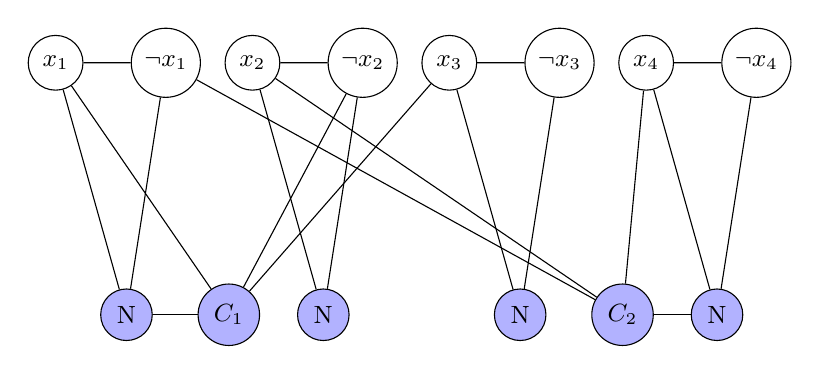
\begin{tikzpicture}[scale=1.0, every node/.style={font=\small}]
    % Variable gadgets with more spacing
    \foreach \i/\x in {1/0, 2/2.5, 3/5, 4/7.5} {
        \node[draw,circle,fill=blue!30] (N\i) at (\x,-2) {N};
        \node[draw,circle] (x\i) at (\x-0.9,1.2) {$x_\i$};
        \node[draw,circle] (nx\i) at (\x+0.5,1.2) {$\neg x_\i$};
        \draw (N\i) -- (x\i) -- (nx\i) -- (N\i);
    }

    % Clause gadgets positioned lower and centered between literals
    \node[draw,circle,fill=blue!30] (C1) at (1.3,-2) {$C_1$};
    \node[draw,circle,fill=blue!30] (C2) at (6.3,-2) {$C_2$};
    
    % Connections for C1 = (x1 ∨ ¬x2 ∨ x3)
    \draw (C1) -- (x1);
    \draw (C1) -- (nx2);
    \draw (C1) -- (x3);
    \draw (C1) -- (N1); % base vertex connection

    % Connections for C2 = (¬x1 ∨ x2 ∨ x4)
    \draw (C2) -- (nx1);
    \draw (C2) -- (x2);
    \draw (C2) -- (x4);
    \draw (C2) -- (N4); % base vertex connection
\end{tikzpicture}
\end{center}
\end{frame}

\begin{frame}{Correctness Proof}
    \begin{alertblock}{Key Observation}
    Any valid 3-coloring corresponds to a satisfying assignment, and vice versa.
    \end{alertblock}
    \begin{columns}[T]
        \begin{column}{0.5\textwidth}
            \begin{block}{($\Rightarrow$) Satisfiable $\implies$ 3-colorable}
        \       \begin{itemize}
                    \item Set True variables to \textcolor{green}{T}, False to \textcolor{red}{F}
                    \item Color clauses using remaining color for $C$
                    \item All constraints satisfied
                \end{itemize}
            \end{block}
        \end{column}
        \begin{column}{0.5\textwidth}
            \begin{block}{($\Leftarrow$) 3-colorable $\implies$ Satisfiable}
                \begin{itemize}
                    \item Extract assignment from variable colors
                    \item Each clause has at least one \textcolor{green}{T} literal
                    \item Formula satisfied
                \end{itemize}
            \end{block}
        \end{column}
    \end{columns}
\end{frame}

\begin{frame}{Correctness Proof}
    \begin{alertblock}{Polynomial Time}
        Construction is $O(n+m)$ where:
        \begin{itemize}
            \item $n$ = number of variables
            \item $m$ = number of clauses
        \end{itemize}
    \end{alertblock}

    \begin{exampleblock}{NP-Completeness}
        Proves 3-Coloring is NP-complete via reduction from 3-SAT
    \end{exampleblock}
\end{frame}

\begin{frame}{Dr. Mudassir Shabbir's Figure (3-SAT $\leq_p$ 3-Coloring)}
    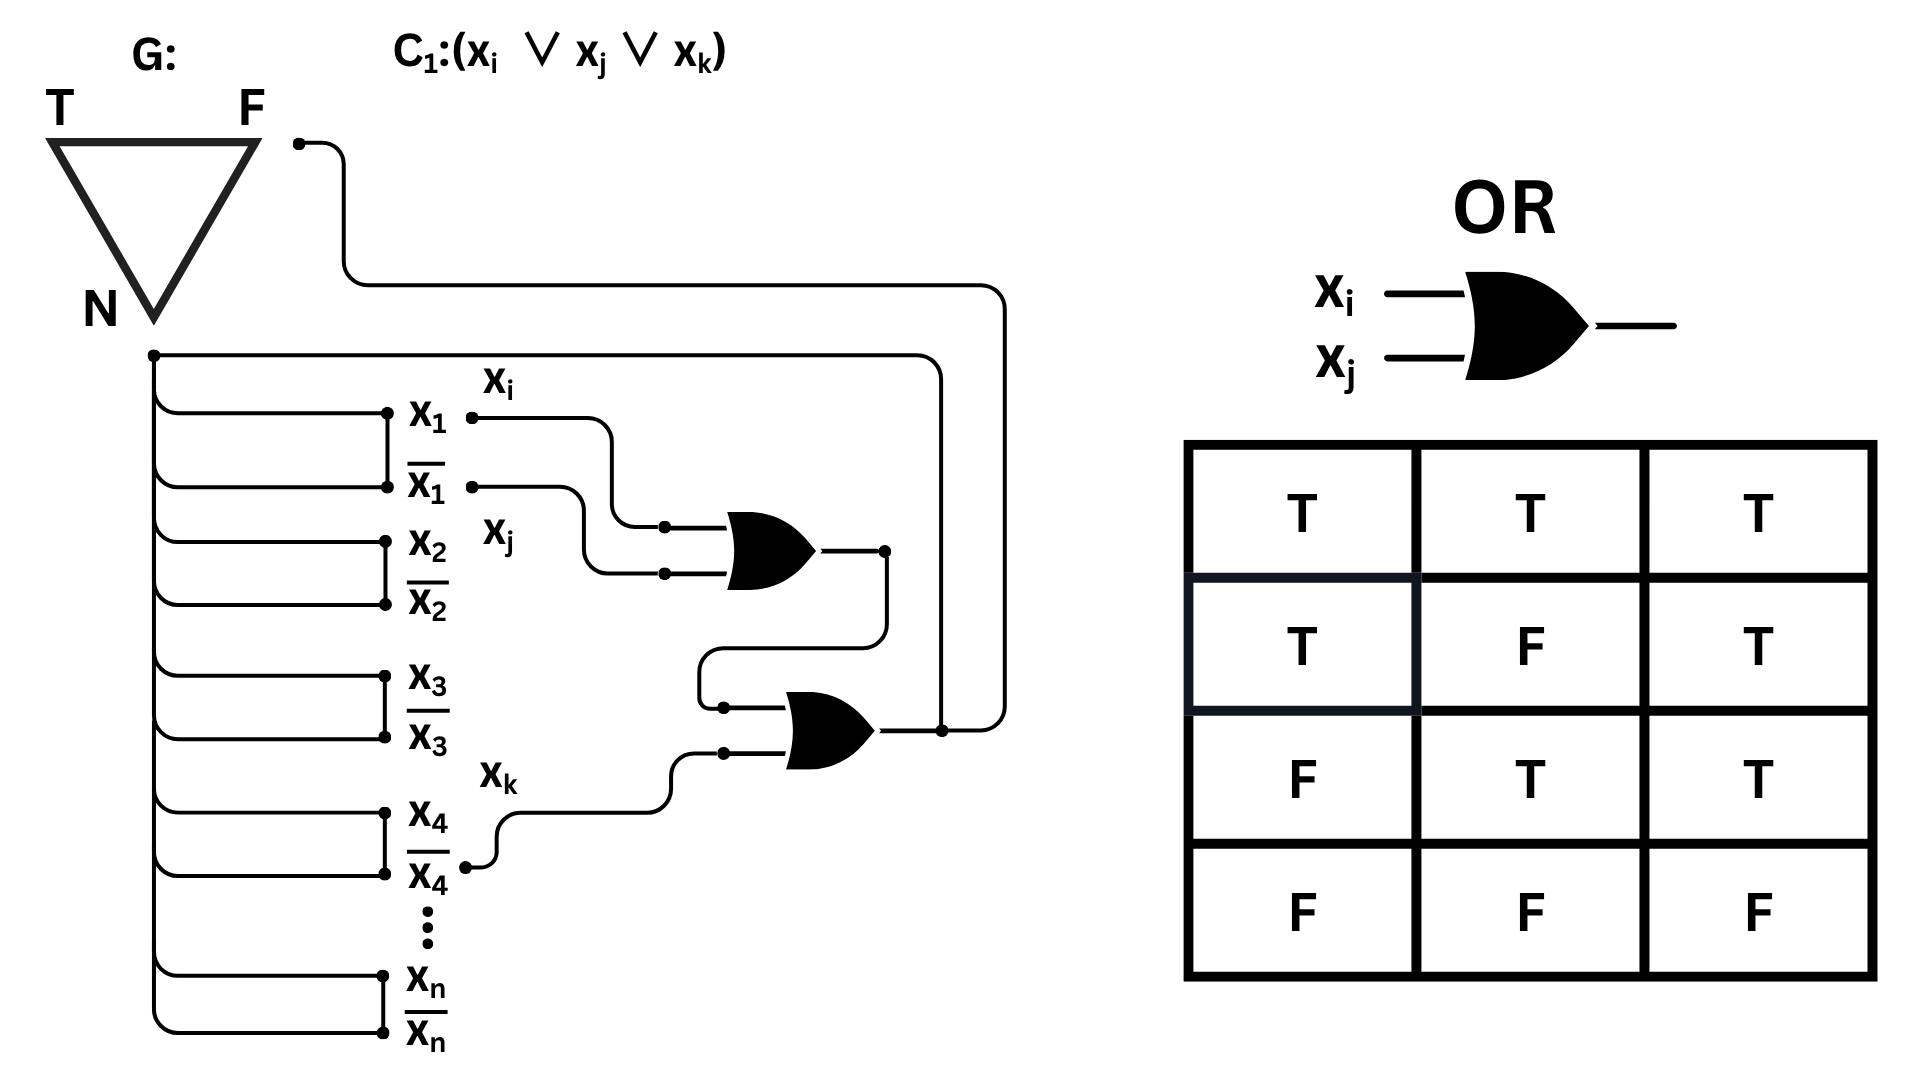
\includegraphics[width={\paperwidth-0.77cm}, height=\paperheight-2.0cm]{Professor's.png}
\end{frame}



\end{document}
